
\chapter{面积}
\label{chap:area}

\section{基本公式}
\label{sec:basic-area-formula}

% \begin{table}[htbp]
%   \centering
%   \renewcommand{\arraystretch}{1.2}
%   % The > directive lets you basically inject the contained code
%   % before each entry in that column.
%   % 
%   % The point of \arraybackslash is to return \\ to its original
%   % meaning because the \centering command alters this and could
%   % possibly give you a noalign error during compilation.
%   % \newcolumntype{C}{ >{\centering\arraybackslash} m{1cm} }
%   % \newcolumntype{D}{ >{\centering\arraybackslash} m{2cm} }
%   % \newcolumntype{E}{ >{\centering\arraybackslash} m{4cm} }
%   % \newcolumntype{F}{ >{\centering\arraybackslash} m{6cm} }

%   % define "struts", as suggested by Claudio Beccari in
%   % a piece in TeX and TUG News, Vol. 2, 1993.
%   % \newcommand\Tstrut{\rule{0pt}{2.6ex}}         % = `top' strut
%   % \newcommand\Bstrut{\rule[-0.9ex]{0pt}{0pt}}   % = `bottom' strut
  
%   \begin{tabular}{cccl}
%     \hline
%     序号&图形 & 示例 & 公式\\
%     \hline\\[2pt]
%     1 & 三角形 & \tikz{\draw(2,2)--(0,0)--(3,0)--(2,2)--(2,0)
%                             (1.8,0)--(1.8,.2)--(2,.2);
%                  \draw[|<->|](0,-.3)--(3,-.3)node[midway,fill=white]{$a$};
%                  \draw[|<->|](3.5, 0)--(3.5, 2)node[midway,fill=white]{$h$};
%                  } & $S=\frac12 ah$\\
%     2 & 矩阵 & \tikz{
%                \draw(0,0)rectangle(3,2);
%                \draw[|<->|](0,-.3)--(3,-.3)node[midway,fill=white]{$a$};
%                \draw[|<->|](3.5,0)--(3.5,2)node[midway,fill=white]{$b$};
%                } & $S=ab$\\
%     \hline
%   \end{tabular}
%   \caption{基本面积公式}
%   \label{tab:basic-area-formula}
% \end{table}

一些基本图形的面积公式列表如下:
\begin{center}
\begin{tikzpicture}
  \begin{scope}[shift={(0,0)}]
    \draw(2,2)--(0,0)--(3,0)--(2,2)--(2,0)
    (1.8,0)--(1.8,.2)--(2,.2);
    \draw[|<->|](0,-.3)--(3,-.3)node[midway,fill=white]{$a$};
    \draw[|<->|](3.5, 0)--(3.5, 2)node[midway,fill=white]{$h$};
    \node[right]at (4,1){$S=\dfrac12 ah$};
  \end{scope}

  \begin{scope}[shift={(8,0)}]
    \draw(0,0)rectangle(3,2);
    \draw[|<->|](0,-.3)--(3,-.3)node[midway,fill=white]{$a$};
    \draw[|<->|](3.5,0)--(3.5,2)node[midway,fill=white]{$b$};
    \node[right]at (4,1){$S=ab$};
  \end{scope}

  \begin{scope}[shift={(0,-4)}]
    \draw[|<->|](1,2.3)--(2.5,2.3)node[midway,fill=white]{$b$};
    \draw[|<->|](0,-.3)--(3,-.3)node[midway,fill=white]{$a$};
    \draw[|<->|](3.5,0)--(3.5,2)node[midway,fill=white]{$h$};
    \draw(0,0)--(3,0)--(2.5,2)--(1,2)--cycle;
    \node[right]at (4,1){$S=\dfrac12 (a+b)h$};
  \end{scope}

  \begin{scope}[shift={(8,-4)}]
    \draw(1.5,1)circle(1.5);
    \draw[->](1.5,1)--(3,1)node[midway,above]{$r$};
    \node[right]at(4,1){$S=\pi r^2$};
  \end{scope}

  \begin{scope}[shift={(0,-8)}]
    \draw(0,1)node(O){}--(3,1)node(A){} arc(0:30:3) node(B){}--cycle;
    \draw[|<->|](0,.6)--(3,.6)node[midway,below]{$r$};
    \draw pic["$\theta$",<->,draw=orange,angle eccentricity=1.6,angle radius=.6cm]{angle=A--O--B};
    \node[right]at(4,1.5){$S=\dfrac12 \theta r^2$};
  \end{scope}
\end{tikzpicture}
\end{center}

\begin{example}
  已知正方形边长,求阴影面积。

  \centering
  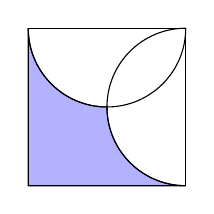
\begin{tikzpicture}[scale=2.0]
    \draw[fill=blue!30](0,0)--(1,0)arc(-90:-180:.5)arc(-90:-180:.5)--cycle;
    \draw(0,0)--(1,0)--(1,1)--(0,1)--cycle;
    \draw(1,0)arc(-90:-270:.5) (1,1)arc(0:-180:.5);
  \end{tikzpicture}
\end{example}

\hints 作辅助线,分别求各部分面积。

\begin{center}
  \begin{tikzpicture}[scale=2.0]
    % \draw[fill=blue!30](0,0)--(1,0)arc(-90:-180:.5)arc(-90:-180:.5)--cycle;
    \draw(0,0)--(1,0)--(1,1)--(0,1)--cycle;
    \draw(1,0)arc(-90:-270:.5) (1,1)arc(0:-180:.5);
    \draw[dashed,pattern=north east lines,pattern color=blue!30](.5,.5)rectangle(1,1);
  \end{tikzpicture}
\end{center}

\begin{example}
  求阴影面积

  \centering
  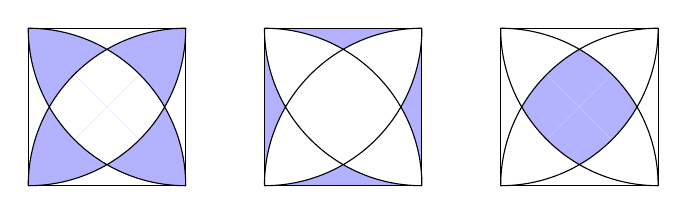
\begin{tikzpicture}[scale=1.0]
    \begin{scope}[shift={(0,0)}]
      \draw(0,0)rectangle(2,2);
      \draw[fill=blue!30,even odd rule]
           ([shift=(0:2)]0,0)arc(0:90:2)
           ([shift=(90:2)]2,0)arc(90:180:2)
           ([shift=(180:2)]2,2)arc(180:270:2)
           ([shift=(270:2)]0,2)arc(270:360:2);
    \end{scope}

    \begin{scope}[shift={(3,0)}]
      \fill[color=blue!30] (0,0)--(2,0) arc(-90:-120:2) arc(-60:-90:2);
      \fill[color=blue!30] (2,0)--(2,2) arc(0:-30:2) arc(30:0:2);
      \fill[color=blue!30] (2,2)--(0,2) arc(90:60:2) arc(120:90:2);
      \fill[color=blue!30] (0,2)--(0,0) arc(180:150:2) arc(210:180:2);
      \draw(0,0)rectangle(2,2);
      \draw([shift=(0:2)]0,0)arc(0:90:2)
           ([shift=(90:2)]2,0)arc(90:180:2)
           ([shift=(180:2)]2,2)arc(180:270:2)
           ([shift=(270:2)]0,2)arc(270:360:2);
    \end{scope}

    \begin{scope}[shift={(6,0)}]
      \fill[color=blue!30]
           ([shift=(0:2)]0,0)arc(0:90:2)
           ([shift=(90:2)]2,0)arc(90:180:2)
           ([shift=(180:2)]2,2)arc(180:270:2)
           ([shift=(270:2)]0,2)arc(270:360:2);
      \fill[color=white,even odd rule]
           ([shift=(0:2)]0,0)arc(0:90:2)
           ([shift=(90:2)]2,0)arc(90:180:2)
           ([shift=(180:2)]2,2)arc(180:270:2)
           ([shift=(270:2)]0,2)arc(270:360:2);
      \draw(0,0)rectangle(2,2);
      \draw([shift=(0:2)]0,0)arc(0:90:2)
           ([shift=(90:2)]2,0)arc(90:180:2)
           ([shift=(180:2)]2,2)arc(180:270:2)
           ([shift=(270:2)]0,2)arc(270:360:2);
    \end{scope}
  \end{tikzpicture}
\end{example}
\begin{proof}[解]
  交点将圆弧平均分成三段,每段对应于$30^\circ$的圆弧。\hints 图中三角形是等边三角形。

  \begin{center}
  \begin{tikzpicture}[scale=1.0]
    \draw(0,0)rectangle(2,2);
    \draw([shift=(0:2)]0,0)arc(0:90:2)
         ([shift=(90:2)]2,0)arc(90:180:2)
         ([shift=(180:2)]2,2)arc(180:270:2)
         ([shift=(270:2)]0,2)arc(270:360:2);
    \coordinate (A) at (60:2);
    \draw[very thick](0,0)--(2,0)--(A)--cycle;
    \fill[pattern=north west lines,pattern color=blue!30](0,0)--(A)arc(60:90:2)--cycle;
    \fill[pattern=north east lines,pattern color=blue!30](2,0)--(2,2)arc(90:120:2)--cycle;
  \end{tikzpicture}
  \end{center}

  可按图中分割方式求解题目第二个图中阴影面积。
\end{proof}

\begin{example}
  由两个圆弧组成的图形称为半月形(lune)。求图中阴影部分半月形的面积。

  \centering
  \begin{tikzpicture}[scale=1.5]
    \coordinate (O) at (0,0);
    \coordinate (A) at (120:1); 
    \coordinate (B) at (60:1);
    \coordinate (C) at ($.5*(A) + .5*(B)$);
    \draw[fill=blue!30](B)arc(0:180:.5);
    \draw[fill=white](1,0)arc(0:180:1);
    \draw[dashed](A)--(B) node[midway,below]{$1$};
    \draw(-1,0)--(1,0) node[midway, below]{$2$};;
  \end{tikzpicture}
\end{example}
\begin{proof}[提示]
  可转换为求弓形面积。

  \begin{center}
    \begin{tikzpicture}[scale=2.0]
      \coordinate (O) at (0,0);
      \coordinate (A) at (120:1);
      \coordinate (B) at (60:1);
      \draw[pattern=north west lines, pattern color=blue!30](A)--(B) arc(60:120:1);
      \draw(A)--(O)--(B);
    \end{tikzpicture}
  \end{center}

  弓形面积可由上图中分割方式求出,即扇形面积减三角形面积。
\end{proof}

\begin{example}
  图中四边形为单位正方形,求阴影面积。

  \centering
  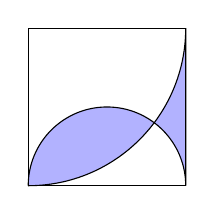
\begin{tikzpicture}[scale=1.0]
    \draw[fill=blue!30,even odd rule](0,0)arc(-90:0:2)--(2,0)arc(0:180:1);
    \draw(2,0)--(0,0)--(0,2)--(2,2);
  \end{tikzpicture}
\end{example}
\begin{proof}[解]
  除了积分,暂时未发现有其它好方法。(超过中小学知识?)
  \begin{align*}
    S&=\int_{x=0}^1 \left| \sqrt{0.5^2 - (x-0.5)^2} - \left(1-\sqrt{1-x^2}\right)\right| \dx\qedhere
  \end{align*}

  % 假设可以求出大圆弧将小圆弧切割成的两部分,小部分的弧角是$x$,则是可
  % 以求出面积与$x$之间的关系。连接圆弧交点与正方形右下角顶点,可以求得
  % 弓形面积
\end{proof}

\begin{example}
  已知三角形面积为$1$,求阴影面积。其中第一个图的线段长度的比例如图所示。后两图,若其中线段长度的比例都已知,则阴影面积又该如何求解?

  \centering
  \begin{tikzpicture}[scale=1.0]
    \begin{scope}[shift={(0,0)}]
      \coordinate (A) at (1.8,2);
      \coordinate (B) at (0,0);
      \coordinate (C) at (3,0);
      \coordinate (D) at ($.6*(C)$);
      \coordinate (E) at ($2/3*(A)+1/3*(C)$);
      \draw(A)--(B)--(C)--cycle (D)--(E);
      \fill[pattern=north west lines,pattern color=blue!30](C)--(D)--(E)--cycle;

      \coordinate (B') at ($(0,-.4) + (B)$);
      \coordinate (C') at ($(0,-.4) + (C)$);
      \coordinate (D') at ($(0,-.4) + (D)$);
      \draw[|<->|](B')--(D') node[midway,below]{$3x$};
      \draw[|<->|](D')--(C') node[midway,below]{$2x$};

      \coordinate (P)  at ($({.4*2/sqrt(5.44)}, {.4*1.2/sqrt(5.44)})$);
      \coordinate (C') at ($(P) + (C)$);
      \coordinate (E') at ($(P) + (E)$);
      \coordinate (A') at ($(P) + (A)$);
      \draw[|<->|](C')--(E') node[pos=.75,above right,sloped]{$2y$};
      \draw[|<->|](E')--(A') node[pos=.75,above right,sloped]{$y$};
    \end{scope}

    \begin{scope}[shift={(4.5,0)}]
      \coordinate (B) at (0,0);
      \coordinate (C) at (3,0);
      \coordinate (A) at (2,2);
      \coordinate (D) at ($.4*(B) + .6*(C)$);
      \coordinate (E) at ($.3*(A) + .7*(C)$);
      \coordinate (F) at ($.5*(A) + .5*(B)$);
      \draw(A)--(B)--(C)--cycle;
      \draw[pattern=north west lines,pattern color=blue!30](D)--(E)--(F)--cycle;
    \end{scope}

    \begin{scope}[shift={(9,0)}]
      \coordinate (B) at (0,0);
      \coordinate (C) at (3,0);
      \coordinate (A) at (2,2);
      \coordinate (D) at ($.4*(B) + .6*(C)$);
      \coordinate (E) at ($.3*(A) + .7*(C)$);
      \coordinate (F) at ($.5*(A) + .5*(B)$);
      \coordinate (G) at ($.8*(B) + .2*(C)$);
      \draw(A)--(B)--(C)--cycle;
      \draw[pattern=north west lines,pattern color=blue!30](D)--(E)--(F)--(G)--cycle;
    \end{scope}

  \end{tikzpicture}
\end{example}
\begin{proof}[解]\mbox{}\\
  \begin{center}
    \begin{tikzpicture}[scale=1.0]
    \begin{scope}[shift={(0,0)}]
      \coordinate (A) at (1.8,2);
      \coordinate (B) at (0,0);
      \coordinate (C) at (3,0);
      \coordinate (D) at ($.6*(C)$);
      \coordinate (E) at ($2/3*(A)+1/3*(C)$);
      \draw(A)--(B)--(C)--cycle (D)--(E);
      \fill[pattern=north west lines,pattern color=blue!30](C)--(D)--(E)--cycle;

      \coordinate (B') at ($(0,-.4) + (B)$);
      \coordinate (C') at ($(0,-.4) + (C)$);
      \coordinate (D') at ($(0,-.4) + (D)$);
      \draw[|<->|](B')--(D') node[midway,below]{$3x$};
      \draw[|<->|](D')--(C') node[midway,below]{$2x$};

      \coordinate (P)  at ($({.4*2/sqrt(5.44)}, {.4*1.2/sqrt(5.44)})$);
      \coordinate (C') at ($(P) + (C)$);
      \coordinate (E') at ($(P) + (E)$);
      \coordinate (A') at ($(P) + (A)$);
      \draw[|<->|](C')--(E') node[pos=.75,above right,sloped]{$2y$};
      \draw[|<->|](E')--(A') node[pos=.75,above right,sloped]{$y$};

      \draw[dashed](A)--(D);
    \end{scope}
  \end{tikzpicture}
\end{center}

  作辅助线,可以容易看出各个三角形之间的面积关系。
\end{proof}


\begin{example}
  已知正方形边长,求阴影面积。

  \begin{center}
    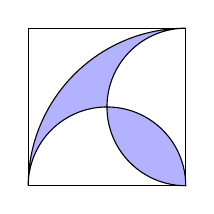
\begin{tikzpicture}[scale=1.0]
      \coordinate(A)at(0,0);
      \coordinate(B)at(2,0);
      \coordinate(C)at(2,2);
      \coordinate(D)at(0,2);
      \draw(A)--(B)--(C)--(D)--cycle;
      \draw[fill=blue!30, even odd rule] (A) arc(180:90:2) arc(90:270:1) arc(0:180:1);
    \end{tikzpicture}
  \end{center}
\end{example}
\begin{proof}[提示]
  变换,如图。
  \begin{center}
    \begin{tikzpicture}[scale=1.0]
      \coordinate(A)at(0,0);
      \coordinate(B)at(2,0);
      \coordinate(C)at(2,2);
      \coordinate(D)at(0,2);
      \draw(A)--(B)--(C)--(D)--cycle;
      \draw[fill=blue!30, even odd rule] (A) arc(180:90:2) arc(90:180:1) arc(90:180:1);
      \fill[pattern=crosshatch, pattern color=red!50](C) arc(90:180:1) arc(90:180:1) -- (C);
      \draw[dashed](A)--(C) (1,1)--(B);
      \draw(B) arc(0:90:1) arc(180:270:1);
    \end{tikzpicture}
  \end{center}

  原阴影面积等于$\frac14$圆减去一个等腰直角三角形。
\end{proof}

\section{面积法}
\label{sec:area-method}

有时解决问题可以升维或降维。比如在某些情况下求解线段问题时,可以升维成面积问题。反之,有时求解体积问题时可以降维成线段问题。

\begin{example}
  如图,$D$和$E$是$\triangle ABC$两边上一点,$O$是$AE$与$CD$的交点。若$\dfrac{CE}{BE}=\dfrac{u}{v}$,$\dfrac{AD}{BD}=\dfrac{x}{y}$,求$\dfrac{CO}{DO}$。
  \begin{center}
    \begin{tikzpicture}[scale=1.5]
      \coordinate[label=below left:$A$](A) at (0,0);
      \coordinate[label=below right:$B$](B) at (3,0);
      \coordinate[label=above:$C$](C) at (2,2);
      \coordinate[label=below:$D$](D) at ($.6*(A)+.4*(B)$);
      \coordinate[label=right:$E$](E) at ($.5*(B)+.5*(C)$);
      \coordinate[label=above left:$O$](O) at ($2/7*(C)+5/7*(D)$);
      \draw(A)--(D) node[midway,below]{$x$};
      \draw(D)--(B) node[midway,below]{$y$};
      \draw(B)--(E) node[midway,right]{$v$};
      \draw(E)--(C) node[midway,right]{$u$};
      \draw(C)--(A)--(O)--(E) (C)--(D);
      \tkzDrawPoints(A,B,C,D,E,O)
    \end{tikzpicture}
  \end{center}
\end{example}
\begin{proof}[提示]利用面积法。如图,设$\triangle AOD$与$\triangle COE$的面积分别为$M$和$N$。
  \begin{center}
    \begin{tikzpicture}[scale=1.5]
      \begin{scope}
        \coordinate[label=below left:$A$](A) at (0,0);
        \coordinate[label=below right:$B$](B) at (3,0);
        \coordinate[label=above:$C$](C) at (2,2);
        \coordinate[label=below:$D$](D) at ($.6*(A)+.4*(B)$);
        \coordinate[label=right:$E$](E) at ($.5*(B)+.5*(C)$);
        \coordinate[label=above left:$O$](O) at ($2/7*(C)+5/7*(D)$);
        \fill[color=red!20](A)--(D)--(O)--cycle;
        \fill[pattern=north west lines](C)--(E)--(O)--cycle;
        \draw(A)--(D) node[midway,below]{$x$};
        \draw(D)--(B) node[midway,below]{$y$};
        \draw(B)--(E) node[midway,right]{$v$};
        \draw(E)--(C) node[midway,right]{$u$};
        \draw(C)--(A)--(O)--(E) (C)--(D);
        \tkzDrawPoints(A,B,C,D,E,O)
        \node at ($1/3*(A)+1/3*(D)+1/3*(O)$) {$M$};
        \node[fill=white,circle] at ($1/3*(C)+1/3*(E)+1/3*(O)$) {$N$};
      \end{scope}
      \begin{scope}[shift={(0,-3)}]
        \coordinate[label=below left:$A$](A) at (0,0);
        \coordinate[label=below right:$B$](B) at (3,0);
        \coordinate[label=above:$C$](C) at (2,2);
        \coordinate[label=below:$D$](D) at ($.6*(A)+.4*(B)$);
        \coordinate[label=right:$E$](E) at ($.5*(B)+.5*(C)$);
        \coordinate[label=above left:$O$](O) at ($2/7*(C)+5/7*(D)$);
        \fill[color=red!20](A)--(D)--(O)--cycle;
        \fill[pattern=north west lines](C)--(E)--(O)--cycle;
        \draw(A)--(D) node[midway,below]{$x$};
        \draw(D)--(B) node[midway,below]{$y$};
        \draw(B)--(E) node[midway,right]{$v$};
        \draw(E)--(C) node[midway,right]{$u$};
        \draw(C)--(A)--(O)--(E) (C)--(D);
        \draw[dashed](B)--(O);
        \tkzDrawPoints(A,B,C,D,E,O)
        \node at ($1/3*(A)+1/3*(D)+1/3*(O)$) {$M$};
        \node[fill=white,circle] at ($1/3*(C)+1/3*(E)+1/3*(O)$) {$N$};
        \node(SBOE) at ($.5*(B)+.5*(E)+(2,0)$) {$S_{\triangle BOE} = \dfrac{v}{u}\cdot N$};
        \node(SBOD) at ($(B)+(-1,-1)$) {$S_{\triangle BOD}=\dfrac{y}{x}\cdot M$};
        \node(SAOC) at ($.5*(A)+.5*(C)+(-2,0)$) {$S_{\triangle AOC}=\dfrac{u}{v}\left(1+\dfrac{y}{x}\right)\cdot M$};
    \end{scope}
    \end{tikzpicture}
  \end{center}
  连接$BO$,可分别求得各部分的面积,即
  \begin{align*}
    &S_{\triangle BOD} = \frac{y}{x}\cdot M,\quad\quad
    S_{\triangle BOE} = \frac{v}{u}\cdot N\\
    \implies& S_{\triangle ABE} = \left(1 + \frac{y}{x}\right)\cdot M + \frac{v}{u}\cdot N \\
    \implies& S_{\triangle ACE} = \frac{u}{v}\cdot S_{\triangle ABE} =
              \frac{u}{v}\left(1+\frac{y}{x}\right)\cdot M + N\\
    \implies& S_{\triangle AOC} = \frac{u}{v}\left(1+\frac{y}{x}\right)\cdot M
  \end{align*}
  由此可得
  \begin{align*}
    \frac{CO}{DO}= & \frac{S_{\triangle AOC}}{S_{\triangle AOD}}= \frac{u}{v}\left(1+\frac{y}{x}\right)
  \end{align*}

  这里还可以得到关于$M$与$N$之间关系的结论。由类似的方法得到$S_{\triangle AOC}$关于$N$的表达式为
  \begin{align*}
    & S_{\triangle AOC} = \frac{x}{y}\left(1+\frac{v}{u}\right)\cdot N\\
    \implies & \frac{u}{v}\left(1+\frac{y}{x}\right)\cdot M = \frac{x}{y}\left(1+\frac{v}{u}\right)\cdot N\qedhere
  \end{align*}
\end{proof}

\begin{example}[正八边形]
  若正八边形最长的对角线为$a$,最短的对角线为$b$,则正八边形的面积是$ab$。
  \begin{center}
    \begin{tikzpicture}[scale=1.0]
      \begin{scope}
        \foreach \i in{0,1,2,3,4,5,6,7}{%
          \coordinate(N\i) at (360/8*\i:2);
        }
        \draw(N0)--(N1)--(N2)--(N3)--(N4)--(N5)--(N6)--(N7)--cycle;
        \draw[help lines](N2)--(N6)node[midway,right]{$a$};
        \draw[help lines](N3)--(N5)node[midway,right]{$b$};
      \end{scope}
      \begin{scope}[shift={(5,0)}]
        \foreach \i in{0,1,2,3,4,5,6,7}{%
          \coordinate(N\i) at (360/8*\i:2);
        }

        \coordinate(A) at ($(N1)!(N0)!(N3)$);
        \coordinate(B) at ($(N1)!(N4)!(N3)$);
        \coordinate(C) at ($(N5)!(N4)!(N7)$);
        \coordinate(D) at ($(N5)!(N0)!(N7)$);
        % \coordinate(E) at ($(N1)!(N2)!(N3)$);
        % \coordinate(F) at ($(N5)!(N6)!(N7)$);
        \fill[red!20](N1)--(N2)--(N3);
        \fill[red!20](N0)--(A)--(N1)--cycle (N3)--(B)--(N4)--cycle;
        \fill[pattern=north west lines,pattern color=blue!20](N5)--(N6)--(N7)--cycle;
        \fill[pattern=north west lines,pattern color=blue!20](N4)--(C)--(N5)--cycle (N7)--(D)--(N0)--cycle;

        \draw[dashed](A)--(B)--(C)--(D)--cycle;
        \draw(N0)--(N1)--(N2)--(N3)--(N4)--(N5)--(N6)--(N7)--cycle;
      \end{scope}
    \end{tikzpicture}
  \end{center}
\end{example}
\begin{proof}[提示]
  由上图,将正八边形切割后可重新拼装成一个$a\times b$的长方形。
\end{proof}

\begin{example}
  如图,$E$是正方形$ABCD$的$AB$边的中点,且阴影面积为$45$,求正方形的面积。
  \begin{center}
    \begin{tikzpicture}[scale=.8]
      \coordinate[label=below left:$A$](A)at(0,0);
      \coordinate[label=below right:$B$](B)at(3,0);
      \coordinate[label=above right:$C$](C)at(3,3);
      \coordinate[label=above left:$D$](D)at(0,3);
      \coordinate[label=below:$E$](E)at($.5*(A)+.5*(B)$);
      \tkzInterLL(B,D)(E,C)\tkzGetPoint{F}
      \fill[color=red!20](A)--(E)--(F)--(D)--cycle;
      \draw(A)--(B)--(C)--(D)--cycle (E)--(C) (D)--(B);
      \tkzLabelPoints[above](F)
      \begin{scope}[shift={(4,0)}]
        \coordinate(A)at(0,0);
        \coordinate(B)at(3,0);
        \coordinate(C)at(3,3);
        \coordinate(D)at(0,3);
        \coordinate(E)at($.5*(A)+.5*(B)$);
        \tkzInterLL(B,D)(E,C)\tkzGetPoint{F}
        % \fill[color=red!20](A)--(E)--(F)--(D)--cycle;
        \fill[pattern=crosshatch,pattern color=red](A)--(F)--(E)--cycle;
        \fill[color=blue!20](F)--(E)--(B)--cycle;
        \draw(A)--(B)--(C)--(D)--cycle (E)--(C) (D)--(B) (A)--(F);
      \end{scope}
      \begin{scope}[shift={(8,0)}]
        \coordinate(A)at(0,0);
        \coordinate(B)at(3,0);
        \coordinate(C)at(3,3);
        \coordinate(D)at(0,3);
        \coordinate(E)at($.5*(A)+.5*(B)$);
        \tkzInterLL(B,D)(E,C)\tkzGetPoint{F}
        % \fill[color=red!20](A)--(E)--(F)--(D)--cycle;
        \fill[pattern=crosshatch,pattern color=red](A)--(F)--(D)--cycle;
        \fill[color=blue!20](C)--(F)--(D)--cycle;
        \draw(A)--(B)--(C)--(D)--cycle (E)--(C) (D)--(B) (A)--(F);
        \draw[dashed](F)--(F |- D) (F)--(F -| D);
      \end{scope}
      \begin{scope}[shift={(12,0)}]
        \coordinate(A)at(0,0);
        \coordinate(B)at(3,0);
        \coordinate(C)at(3,3);
        \coordinate(D)at(0,3);
        \coordinate(E)at($.5*(A)+.5*(B)$);
        \tkzInterLL(B,D)(E,C)\tkzGetPoint{F}
        % \fill[color=red!20](A)--(E)--(F)--(D)--cycle;
        \fill[pattern=crosshatch,pattern color=red](A)--(F)--(B)--cycle;
        \fill[color=blue!20](C)--(F)--(B)--cycle;
        \draw(A)--(B)--(C)--(D)--cycle (E)--(C) (D)--(B) (A)--(F);
        % \draw[dashed](F)--(F |- D) (F)--(F -| D);
      \end{scope}
    \end{tikzpicture}
  \end{center}
\end{example}
\begin{proof}[提示]
  由后面几个图形,由两部分阴影面积相等可以知道只要得出$\triangle DFC$和$\triangle BFC$的面积比,即只要得出$DF:BF$就可以得到图中各种三角形的面积关系,从而由$S_{AEFD}=45$可以求出各个面积。

  \begin{center}
    \begin{tikzpicture}[scale=.8]
      \begin{scope}[shift={(0,0)}]
        \coordinate[label=below left:$A$](A)at(0,0);
        \coordinate[label=below right:$B$](B)at(3,0);
        \coordinate[label=above right:$C$](C)at(3,3);
        \coordinate[label=above left:$D$](D)at(0,3);
        \coordinate[label=below:$E$](E)at($.5*(A)+.5*(B)$);
        \tkzInterLL(B,D)(E,C)\tkzGetPoint{F}
        \coordinate[label=below:$G$](G)at(0,-3);
        % \fill[color=red!20](A)--(E)--(F)--(D)--cycle;
        \fill[pattern=crosshatch,pattern color=red](G)--(F)--(D)--cycle;
        \fill[color=blue!20](C)--(F)--(B)--cycle;
        \draw(A)--(B)--(C)--(D)--cycle (E)--(C) (D)--(B) (A)--(F);
        \draw[dashed](A)--(G)--(E);
        % \draw[dashed](F)--(F |- D) (F)--(F -| D);
        \tkzLabelPoints[above](F)
      \end{scope}      
      \begin{scope}[shift={(5,0)}]
        \coordinate(A)at(0,0);
        \coordinate(B)at(3,0);
        \coordinate(C)at(3,3);
        \coordinate(D)at(0,3);
        \coordinate(E)at($.5*(A)+.5*(B)$);
        \tkzInterLL(B,D)(E,C)\tkzGetPoint{F}
        \draw(A)--(B)--(C)--(D)--cycle (E)--(C) (D)--(B) (A)--(F);
        \node at($1/3*(A)+1/3*(E)+1/3*(F)$){1};
        \node at($1/3*(B)+1/3*(E)+1/3*(F)$){1};
        \node at($1/3*(B)+1/3*(C)+1/3*(F)$){2};
        \node at($1/3*(A)+1/3*(F)+1/3*(D)$){4};
        \node at($1/3*(C)+1/3*(F)+1/3*(D)$){4};
      \end{scope}
    \end{tikzpicture}
  \end{center}
  如上图,延长$CE$与$DA$相交于$G$,可知$AG=BC$,从而$DF:FB=DG:BC=2$。由此可得上面第二图中各面积关系比。
\end{proof}

\begin{example}
  由上面分析,容易得到正方形一个顶点与两条不相邻边的中点的连线将一条对角线三等分。
  \begin{center}
    \begin{tikzpicture}
      \begin{scope}
        \coordinate(A)at(0,0);
        \coordinate(B)at(3,0);
        \coordinate(C)at(3,3);
        \coordinate(D)at(0,3);
        \coordinate(E)at($.5*(A)+.5*(B)$);
        \coordinate(F)at($.5*(A)+.5*(D)$);
        \draw(A)--(B)--(C)--(D)--cycle (E)--(C)--(F) (D)--(B);
      \end{scope}      
    \end{tikzpicture}
  \end{center}
\end{example}


\section{Primary Skill}
\label{sec:primary-skill-in-calculating-area}

\begin{example}
  $AE=EF=FB$, $AG=2GC$, $S_{\triangle EFG}=8$. Find the area of the parallelogram.

  \centering
  \begin{tikzpicture}[scale=2.0]
    \coordinate[label=below left:$A$] (A) at(0,0);
    \coordinate[label=below right:$B$](B) at(3,0);
    \coordinate[label=above right:$C$](C) at(4,2);
    \coordinate[label=above left:$D$] (D) at(1,2);
    \coordinate[label=below:$E$]      (E) at(1,0);
    \coordinate[label=below:$F$]      (F) at(2,0);
    \coordinate[label=above left:$G$] (G) at($1/3*(A)+2/3*(C)$);
    \draw(A)--(B)--(C)--(D)--(A)--(C);
    \filldraw[pattern=north west lines, pattern color=black](E)--(F)--(G)--cycle;
  \end{tikzpicture}
\end{example}

\begin{proof}[Hint]
  Using propotion.

  \begin{center}
    \begin{tikzpicture}[scale=1.0]
      \begin{scope}
        \coordinate(A) at(0,0);
        \coordinate(B) at(3,0);
        \coordinate(C) at(4,2);
        \coordinate(D) at(1,2);
        \coordinate(E) at(1,0);
        \coordinate(F) at(2,0);
        \coordinate(G) at($1/3*(A)+2/3*(C)$);
        \draw(A)--(B)--(C)--(D)--(A)--(C);
        \filldraw[pattern=north west lines, pattern color=black](E)--(F)--(G)--cycle;
        \node at ($1/3*(E)+1/3*(F)+1/3*(G)$) {$8$};
      \end{scope}
      \begin{scope}[shift={(5,0)}]
        \coordinate(A) at(0,0);
        \coordinate(B) at(3,0);
        \coordinate(C) at(4,2);
        \coordinate(D) at(1,2);
        \coordinate(E) at(1,0);
        \coordinate(F) at(2,0);
        \coordinate(G) at($1/3*(A)+2/3*(C)$);
        \draw(A)--(B)--(C)--(D)--(A)--(C);
        \filldraw[pattern=north west lines, pattern color=black](A)--(B)--(G)--cycle;
        \node at ($1/3*(A)+1/3*(B)+1/3*(G)$) {$24$};
      \end{scope}
      \begin{scope}[shift={(10,0)}]
        \coordinate(A) at(0,0);
        \coordinate(B) at(3,0);
        \coordinate(C) at(4,2);
        \coordinate(D) at(1,2);
        \coordinate(E) at(1,0);
        \coordinate(F) at(2,0);
        \coordinate(G) at($1/3*(A)+2/3*(C)$);
        \draw(A)--(B)--(C)--(D)--(A)--(C);
        \filldraw[pattern=north west lines, pattern color=black](A)--(B)--(C)--cycle;
        \node at ($1/3*(A)+1/3*(B)+1/3*(C)$) {$36$};
      \end{scope}
    \end{tikzpicture}
  \end{center}
\end{proof}


\begin{example}
  Knowing $D,E$ are the middle point of $BC$ and $CA$ respectively, and $S_{\triangle ABC}=60$, find the area of the shadow $\triangle ABO$.
  \centering
  \begin{tikzpicture}[scale=2.0]
    \foreach \n/\x/\y/\p in{A/0/0/below left, B/3/0/below right, C/2/2/above}{
      \coordinate[label=\p:$\n$](\n)at(\x,\y);
    }
    \coordinate[label=above right:$D$](D)at($.5*(B)+.5*(C)$);
    \coordinate[label=above left:$E$](E)at($.5*(A)+.5*(C)$);
    \draw(A)--(B)--(C)--(A)--(D)
         (B)--(E);
    \tkzInterLL(A,D)(B,E)\tkzGetPoint{O}
    \tkzLabelPoints[above](O)
    \filldraw[pattern=north west lines, pattern color=black](A)--(O)--(B)--cycle;
  \end{tikzpicture}
\end{example}

\begin{proof}[Hint]
  The three parts have the same area. Or, the six parts have the same area.
  \begin{center}
    \begin{tikzpicture}[scale=1.5]
      \begin{scope}
        \foreach \n/\x/\y/\p in{A/0/0/below left, B/3/0/below right, C/2/2/above}{
          \coordinate[label=\p:$\n$](\n)at(\x,\y);
        }
        \coordinate(O)at($1/3*(A)+1/3*(B)+1/3*(C)$);
        \draw(A)--(B)--(C)--(A)--(O)--(B) (O)--(C);
        \fill[color=red!10](A)--(O)--(C);
        \fill[pattern=north west lines, pattern color=black](A)--(O)--(B);
        \fill[pattern=north east lines, pattern color=black](C)--(O)--(B);
      \end{scope}
      \begin{scope}[shift={(4,0)}]
        \foreach \n/\x/\y/\p in{A/0/0/below left, B/3/0/below right, C/2/2/above}{
          \coordinate[label=\p:$\n$](\n)at(\x,\y);
        }
        \coordinate(D)at($.5*(B)+.5*(C)$);
        \coordinate(E)at($.5*(C)+.5*(A)$);
        \coordinate(F)at($.5*(A)+.5*(B)$);
        \coordinate(O)at($1/3*(A)+1/3*(B)+1/3*(C)$);
        \draw(A)--(B)--(C)--(A)--(D) (B)--(E) (C)--(F);
        \fill[color=red!10](A)--(O)--(F)--cycle
                           (B)--(O)--(D)--cycle
                           (C)--(O)--(E)--cycle;
      \end{scope}
    \end{tikzpicture}
  \end{center}
\end{proof}


\begin{example}
  求图中阴影部分面积,其中的三角形是直角三角形。

  \centering
  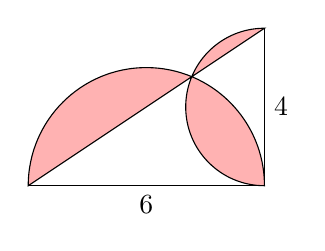
\begin{tikzpicture}[scale=0.5]
    \draw[fill=red!30, even odd rule](0,0) arc(180:0:3) arc(270:90:2) --cycle;
    \draw(0,0)--(6,0)node[midway, below]{$6$} -- (6,4)node[midway, right]{$4$};
  \end{tikzpicture}
\end{example}
\begin{proof}[提示]
  大半圆 + 小半圆 = 三角形 + 阴影
\end{proof}


\begin{question}
  图中四边形是直角梯形,求其中两部分阴影面积的差。
  \begin{center}
    \begin{tikzpicture}[scale=1.0]
      \coordinate(A)at(0,0);
      \coordinate(B)at(8,0);
      \coordinate(C)at(2,6);
      \coordinate(D)at(0,6);
      \begin{scope}
        \clip (A)arc(180:135:8)--(B)--cycle;
        \fill[pattern=north west lines, pattern color=red!70](D)arc(180:315:2)--(C)--cycle;
      \end{scope}
      \begin{scope}
        \clip(A)--(D)arc(180:315:2)--(B)--(A);
        \fill[color=blue!20](A)arc(180:135:8)--(C)--(D)--cycle;
      \end{scope}
      \draw(A)--(B)node[midway, below]{8}--(C)--(D)node[midway,above]{2}--(A)node[midway, left]{6};
      \draw(A)arc(180:135:8) (D)arc(180:315:2);
      \node[draw,circle](none)at(1,5.3){\small $3$};
      \node[fill=white,draw,circle](none)at(0.5,3.9){\small $1$};
      \node[fill=white,draw,circle](none)at(2.2, 4.7){\small $2$};
      \tkzMarkRightAngle(B,A,D)
      \tkzMarkRightAngle(A,D,C)
    \end{tikzpicture}
  \end{center}
\end{question}
\begin{proof}[提示]
  记编号1、2、3的区域面积分别为$S_1, S_2, S_3$,则$S_1$与$S_2$的面积差与两者分别加上$S_3$之后的面积差相等,即
  \begin{align*}
    |S_1 - S_2| = |(\underline{S_1 + S_3}) - (\uwave{S_2 + S_3})|
  \end{align*}
  而$S_1+S_3$及$S_2+S_3$都容易求得。
\end{proof}


\begin{question}
  已知圆半径1,求阴影面积。
  \begin{center}
    \begin{tikzpicture}[scale=0.5]
      \coordinate(A)at(0,0);
      \coordinate(B)at(2,0);
      \coordinate(C)at($(A)!1!60:(B)$);
      \coordinate(D)at($(A)!1!60:(C)$);
      \fill[color=red!50](A)arc(240:180:2)arc(120:60:2)arc(120:180:2);
      \fill[color=red!50](A)arc(180:240:2)arc(300:360:2)arc(300:240:2);
      \fill[color=red!50](B)arc(300:360:2)arc(60:120:2)arc(60:0:2);
      \draw(A)circle(2);
      \draw(B)circle(2);
      \draw(C)circle(2);
    \end{tikzpicture}
  \end{center}
\end{question}
\begin{proof}[提示]
  作辅助线。
  \begin{center}
    \begin{tikzpicture}[scale=0.5]
      \coordinate(A)at(0,0);
      \coordinate(B)at(2,0);
      \coordinate(C)at($(A)!1!60:(B)$);
      \coordinate(D)at($(A)!1!60:(C)$);
      \fill[color=red!50](A)arc(240:180:2)--(C)--(A);
      \fill[color=red!50](A)arc(180:240:2)arc(300:360:2)arc(300:240:2);
      \fill[color=red!50](B)arc(300:360:2)arc(60:120:2)arc(60:0:2);
      \draw(A)circle(2);
      \draw(B)circle(2);
      \draw(C)circle(2);
      \draw[dashed](D)--(C)--(A);
    \end{tikzpicture}
  \end{center}
  可知,每个阴影的面积等于一个$60^\circ$的扇形面积,三个加起来等于半个圆。
\end{proof}


\begin{question}
  如图,一个单位圆和等腰直角三角形,求其中阴影面积。
  \begin{center}
    \begin{tikzpicture}[scale=1.0]
      \begin{scope}
        \draw[fill=blue!30,even odd rule](0,0) arc(0:360:1) -- (-2,0)--(0,2)--cycle;
      \end{scope}
      \begin{scope}[shift={(2,0)}]
        \coordinate(O) at (0,0);
        \coordinate(A) at (1,0);
        \coordinate(B) at (-1,0);
        \coordinate(C) at (1,2);
        \coordinate(D) at ($(C)!1!-45:(A)$);
        \coordinate(E) at (0,1);
        \fill[color=blue!30](O)circle(1);
        \fill[color=white](B)--(A) arc(270:225:2) -- cycle;
        \draw(A)arc(0:360:1)--(C)--(B)--cycle (A) arc(270:225:2);
      \end{scope}
    \end{tikzpicture}
  \end{center}
\end{question}
\begin{proof}[提示]
  先求圆内空白部分面积。
\end{proof}

\begin{example}
  如图,$\triangle ABC$与$\triangle ADE$都是边长为3的正三角形,$\angle DAC=30^\circ$。求图中阴影部分面积。

  \centering
  \begin{tikzpicture}[scale=1.0]
    \coordinate[label=above:$A$] (A) at (0,0);
    \coordinate[label=left:$B$] (B) at (225:3);
    \coordinate[label=left:$D$] (D) at (255:3);
    \coordinate[label=right:$C$] (C) at (285:3);
    \coordinate[label=right:$E$] (E) at (315:3);
    \coordinate[label=below:$F$] (F) at ($0.25*(B)+0.75*(C)$);
    \coordinate[label=above left:$O$] (O) at ($0.5*(B) + 0.5*(C)$);
    \fill[color=blue!10](A)--(D)--(F)--(C)--cycle;
    \draw(A)--(B)--(C)--cycle (A)--(D)--(E)--cycle;
  \end{tikzpicture}
\end{example}
\begin{proof}[提示]
  容易看出来,$AF$是整个图形的一个对称轴,从而$AF$是阴影角$\angle DAC$的角平分线,从而角平分线的性质,可以求得$DF$与$CF$的长度,从而可得阴影部分面积。

  也可以利用特殊直角三角形的性质。$\triangle ACF$与$\triangle ADF$都是边长为$3$的三角形,设其高$OF$为$x$,则由有一个$60^\circ$角的直角三角形$ODF$,有
  \begin{align*}
    DF = CF = \frac2{\sqrt3} x
  \end{align*}
  且由$BC = 2 OC$及$OC = OF +FC$,可知
  \begin{align*}
    x + \frac2{\sqrt3} x = \frac32
  \end{align*}
  从而可得$OF$。
\end{proof}


\section{数形结合}
\label{sec:combine-number-and-figure}

\begin{example}[希望杯]
  已知$a>0$,$b>0$,求以$\sqrt{a^2+b^2}$、$\sqrt{a^2+4b^2}$和$\sqrt{4a^2+b^2}$为边长的三角形的面积。
\end{example}
\begin{proof}[提示]
  已知三个边长的情况下,首先想到可用海伦公式求三角形面积
  \begin{align*}
    S=\sqrt{p(p-a)(p-b)(p-c)}
  \end{align*}
  其中$p=(a+b+c)/2$是半周长。然而这个计算量会非常大。

  根据边长的形式,可以考虑勾股定理
  \begin{center}
    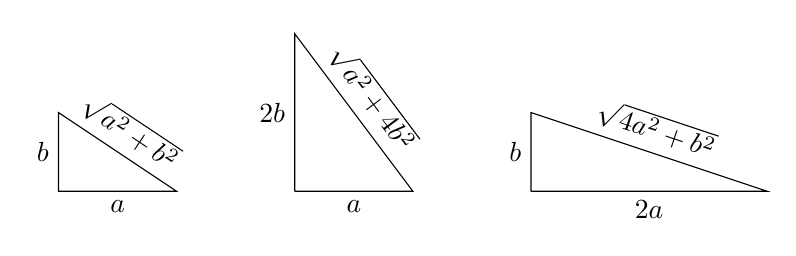
\begin{tikzpicture}[scale=0.5]
      \begin{scope}
        \draw(0,0)--(3,0)node[midway,below]{$a$}--(0,2) node[midway,sloped,above]{$\sqrt{a^2+b^2}$}--cycle node[midway,left]{$b$};
      \end{scope}
      \begin{scope}[shift={(6,0)}]
        \draw(0,0)--(3,0)node[midway,below]{$a$}--(0,4) node[midway,sloped,above]{$\sqrt{a^2+4b^2}$}--(0,0) node[midway,left]{$2b$};
      \end{scope}
      \begin{scope}[shift={(12,0)}]
        \draw(0,0)--(6,0)node[midway,below]{$2a$}--(0,2) node[midway,sloped,above]{$\sqrt{4a^2+b^2}$}--(0,0) node[midway,left]{$b$};
      \end{scope}
    \end{tikzpicture}
  \end{center}
  画到网格上,可以得到下面的图形
  \begin{center}
    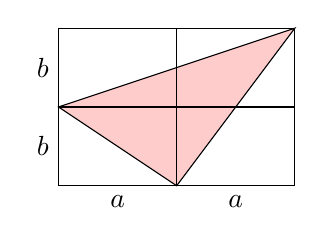
\begin{tikzpicture}[scale=0.5]
      \draw[fill=red!20](3,0)--(0,2)--(6,4)--cycle;
      \draw(0,0)--(3,0)node[midway,below]{$a$}--(6,0)node[midway,below]{$a$}--(6,4)--(0,4)--
           (0,2)node[midway,left]{$b$} --cycle node[midway,left]{$b$}
           (3,0)--(3,4) (0,2)--(6,2);
    \end{tikzpicture}
  \end{center}
  通过空白区域的面积,容易求得图中阴影三角形的面积。
\end{proof}

\begin{question}
  已知$a>0$,$b>0$,求以$\sqrt{a^2+b^2}$、$\sqrt{a^2+9b^2}$和$\sqrt{4a^2+4b^2}$为边长的三角形的面积。
\end{question}





\section{Misc}
\label{sec:misc}

\begin{example}
  Given a square with size $6\times6$ and a rectangle with size $3\times2$, find out the area difference of those not overlapped.

  \centering
  \begin{tikzpicture}[scale=1.0]
    \draw(0,0) rectangle(6,6);
  \end{tikzpicture}
\end{example}


\begin{example}
  % https://math.stackexchange.com/questions/1544719/point-in-the-interior-of-a-square
  A point in the interior of a square $ABCD$ is at distances 3, 4 and meters from the vertices $A$, $B$ and $C$, respectively. What's the area of $ABCD$?
\end{example}


\begin{example}[Same length of side, different height]
  Any point $P$ in the interior of a square $ABCD$, $S_{\triangle ABP} + S_{\triangle CDP}
  = S_{\triangle ACP} + S_{\triangle BDP}$.

  $\triangle ABP$ and $\triangle CDP$ both have a side the length of which is the that of the square, and the heights of them sum up to the length of square too, which makes the sum of the area of the two triangle the half of the square.
  

  Any point $P$ in the interior of square, connect it with the middle points each side. It split into two parts each of which sums to the same area.

  \begin{center}
    \begin{tikzpicture}[scale=1.0]
      \begin{scope}[shift={(0,0)}]
        \coordinate(A)at(0,0);
        \coordinate(B)at(2,0);
        \coordinate(C)at(2,2);
        \coordinate(D)at(0,2);
        \coordinate(P)at(0.7,1.1);
        \draw(A)--(B)--(C)--(D)--(A)--(P)--(B) (C)--(P)--(D);
        \fill[color=blue!20](A)--(P)--(D)--cycle;
        \fill[color=blue!20](B)--(P)--(C)--cycle;
      \end{scope}
      \begin{scope}[shift={(4,0)}]
        \coordinate(A)at(0,0);
        \coordinate(B)at(2,0);
        \coordinate(C)at(2,2);
        \coordinate(D)at(0,2);
        \coordinate(P)at(0.7,1.1);
        \coordinate(E)at($0.5*(A)+0.5*(B)$);
        \coordinate(F)at($0.5*(B)+0.5*(C)$);
        \coordinate(G)at($0.5*(C)+0.5*(D)$);
        \coordinate(H)at($0.5*(D)+0.5*(A)$);
        \draw(A)--(B)--(C)--(D)--cycle (E)--(P)--(F) (G)--(P)--(H);
        \fill[color=blue!20](A)--(E)--(P)--(H)--cycle;
        \fill[color=blue!20](C)--(G)--(P)--(F)--cycle;
      \end{scope}
    \end{tikzpicture}
  \end{center}
\end{example}

\begin{example}
  Any trapezoid $ABCE$ where $AB\parallel CD$, the two diaganl intersects in $P$, then $S_{\triangle ADP}=S_{\triangle BCP}$.
\end{example}


\begin{example}
  $\triangle ABC$, $AB$, $AC$ split into 5 parts equally. The area of the shadow region is 21. What's the area of the triangle?

  \begin{tikzpicture}
    \coordinate[label=left:$A$](A)at(0,0);
    \coordinate[label=below right:$B$](B)at(4,0);
    \coordinate[label=above right:$C$](C)at(3,2);
    \foreach \x/\y/\s in{4/1/5,3/2/5,2/3/5,1/4/5}{%
      \coordinate(B\y)at($\x/\s*(A)+\y/\s*(B)$);
      \coordinate(C\y)at($\x/\s*(A)+\y/\s*(C)$);
    }
    \foreach \a/\b/\c in{A/B1/C1, B1/B2/C2, B2/B3/C3, B3/B4/C4, B4/B/C}{%
      \fill[color=blue!20](\a)--(\b)--(\c)--cycle;
    }
    \draw(C)--(A)--(B)--(C)--(B4)--(C4)--(B3)--(C3)--(B2)--(C2)--(B1)--(C1);
  \end{tikzpicture}
\end{example}

\begin{example}
  Circle with radius 1, find the area of the shadow region.

  \begin{center}
    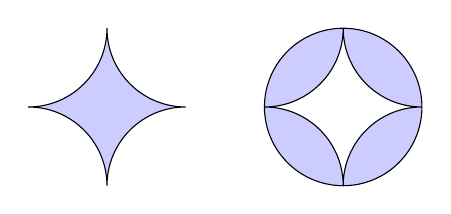
\begin{tikzpicture}[scale=1.0]
      \begin{scope}[shift={(0,0)}]
        \filldraw[black, fill=blue!20](-1,0) arc(-90:0:1) arc(180:270:1) arc(90:180:1) arc(0:90:1);
      \end{scope}
      \begin{scope}[shift={(3,0)}]
        \filldraw[black, fill=blue!20](0,0)circle(1);
        \filldraw[black, fill=white](-1,0) arc(-90:0:1) arc(180:270:1) arc(90:180:1) arc(0:90:1);
      \end{scope}
    \end{tikzpicture}
  \end{center}
\end{example}

Draw an auxilary square like the following
\begin{center}
  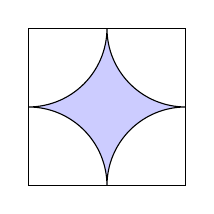
\begin{tikzpicture}
    \filldraw[black, fill=blue!20](-1,0) arc(-90:0:1) arc(180:270:1) arc(90:180:1) arc(0:90:1);
    \draw(-1,-1)rectangle(1,1);
  \end{tikzpicture}
\end{center}
Then the area of the shadow is that of the square subtracted by the 4 quater-of-circle, i.e.,
\begin{align*}
  S_{\text{shadow}} =& S_{\text{square}} - 4\times S_{\text{quarter of square}}\\
  =& 2\times2 - \pi \times 1\times 1 = 4-\pi
\end{align*}
